\chapter{Introduction}
\label{ch:introduction}

\section{Foundations of Digital Trust}

For millennia, the art of secret communication relied on an arms race between the ingenuity of code-makers and the persistence of code-breakers. From the simple substitution ciphers of antiquity, such as the Caesar cipher (Figure~\ref{fig:caesar_cipher}), to the intricate electromechanical rotor machines of the Second World War, security historically depended on the secrecy of the method and the physical complexity of the device.

\begin{figure}[htbp]
    \centering
    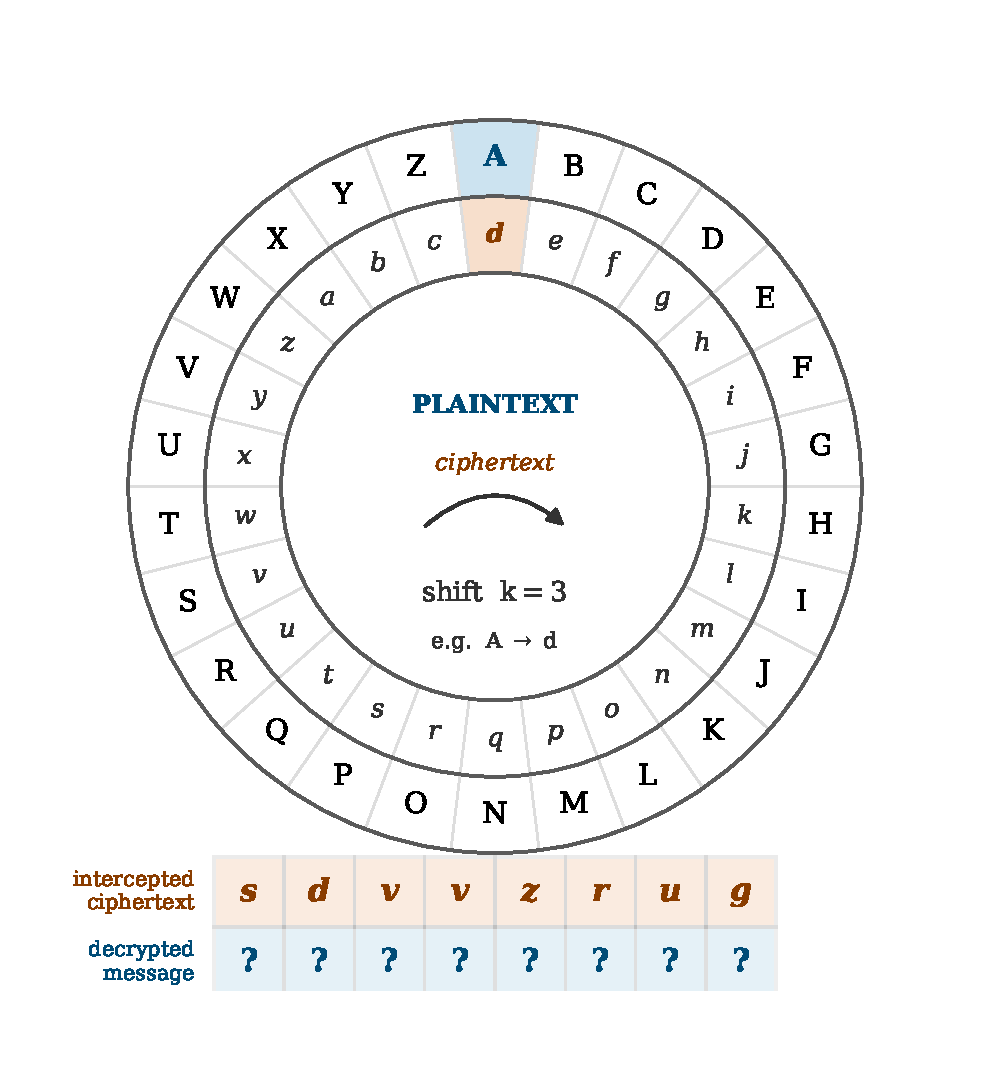
\includegraphics[width=0.62\textwidth]{figures/chapter1/caesar_cipher.pdf}
    \caption{The cipher disk used to encrypt and decrypt with the Caesar cipher.
    The secret key is simply the shift value $k$ (here $k = 3$). Encryption
    aligns the outer plaintext ring against the inner ciphertext ring, rotated by
    $k$ positions, and replaces each letter of the message with the one it meets
    on the inner ring; decryption is the inverse operation, reading from the inner
    ring back out. Formally, $E_k(x) = (x + k) \bmod 26$ and
    $D_k(y) = (y - k) \bmod 26$. The intercepted ciphertext below is left for the
    reader to recover. Its repeated letter already invites frequency analysis,
    and with only $25$ possible shifts the cipher is trivially brute-forced. A
    modern Advanced Encryption Standard (AES) cipher such as AES-256, by contrast, draws its key from
    $2^{256} \approx 10^{77}$ possibilities.}
    \label{fig:caesar_cipher}
\end{figure}

In the modern digital era, this dynamic stabilized around computational complexity. The bedrock of the internet, global commerce, and secure infrastructure rests on mathematical problems, such as factoring large integers or computing discrete logarithms, that are trivially easy to construct but practically impossible for classical computers to solve.

In late 1994, mathematician Peter Shor disrupted this equilibrium. He demonstrated that a hypothetical quantum computer could efficiently solve these exact mathematical problems, effectively neutralizing the public-key cryptography that secures modern communications~\cite{shor1994algorithms}.
A few weeks later, in January 1995, the author of this dissertation was born. The race was on.

\section{The Quantum Threat}

Over the intervening three decades, that theoretical result has evolved into a global engineering effort. Secure communication infrastructure is now entering a transition in which its foundational cryptographic assumptions can no longer be treated as stable design constants. The anticipated arrival of cryptographically relevant quantum computers (CRQCs) motivates a fundamental shift from classical public-key mechanisms toward two emerging technologies that will be explored in detail throughout this thesis: post-quantum cryptography (PQC) and quantum key distribution (QKD).

\subsection{Q-Day}

In security engineering, a \emph{zero-day} is a vulnerability that can be exploited before any defense exists, so that affected systems are compromised without prior warning. Q-Day is the cryptographic counterpart at global scale: the point at which a CRQC renders the public-key cryptography underpinning modern communication breakable, undermining not an individual system but a trust assumption common to nearly all of them simultaneously.

The exact date cannot be predicted. It depends on advances in scaling logical qubits and quantum error correction that have not yet been achieved, leading to a wide range of published timelines. More significant than any single estimate, however, is the consensus among the experts closest to the hardware. A CRQC within the next one to two decades is increasingly regarded as a realistic prospect rather than a remote one (Figure~\ref{fig:qday_timeline}). While individual forecasts vary, their collective trend is consistent.

Q-Day nevertheless differs from a conventional zero-day in one respect that is central to this dissertation: it is anticipated. Because the break is known in advance, the affected cryptography can be replaced before the capability matures, transforming a potentially abrupt failure into a planned, if time-constrained, migration.

\begin{figure}[htbp]
    \centering
    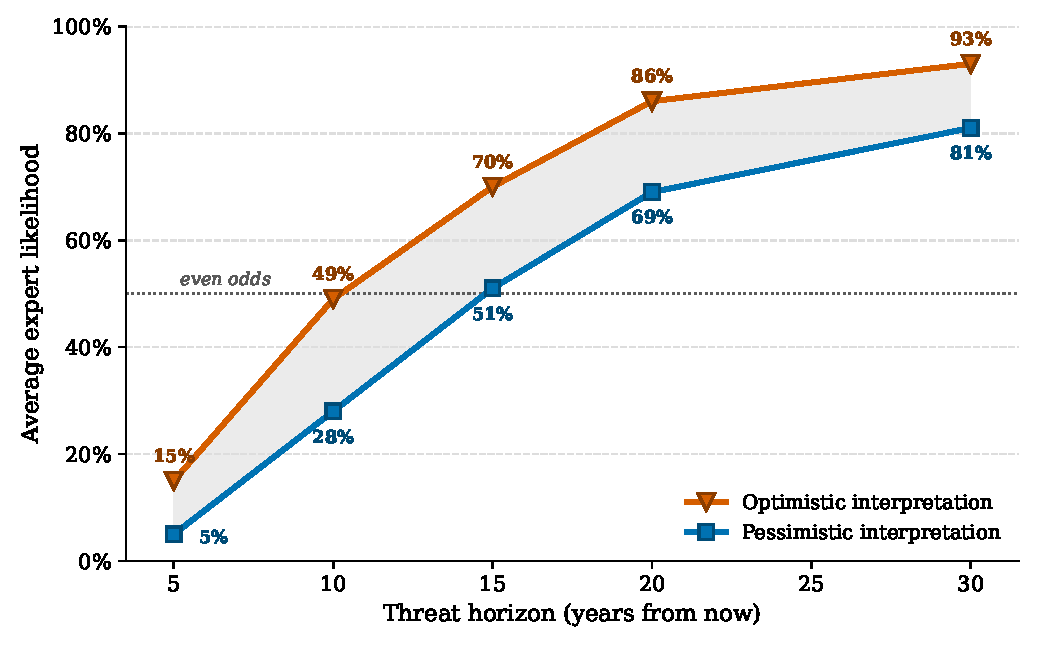
\includegraphics[width=0.8\textwidth]{figures/chapter1/qday_timeline.pdf}
    \caption{Averaged expert likelihood that a quantum computer able to break
    RSA-2048 within 24 hours will exist within a given horizon, under optimistic
    and pessimistic interpretations of the survey responses. Data
    from~\cite{mosca2026quantum}.}
    \label{fig:qday_timeline}
\end{figure}

\subsection{The Hardware Gap}

While the threat timeline is accelerating, a substantial gap remains between the state of the art in quantum hardware and the scale required for cryptanalysis. Breaking a standard 2048-bit RSA key using Shor's algorithm requires a fault-tolerant quantum computer capable of sustaining millions of operations. Historically, this was estimated to require around 20 million physical qubits~\cite{gidney2021factoring}.
However, recent algorithmic optimizations and architectural improvements, such as approximate residue arithmetic, magic state cultivation, and advanced quantum low-density parity check (qLDPC) codes, have drastically reduced these estimates. Current projections suggest that RSA-2048 could be factored in under a week using fewer than one million noisy physical qubits~\cite{gidney2025how}, and potentially under 100,000 physical qubits with next-generation qLDPC architectures~\cite{webster2026pinnacle}.

Despite these theoretical reductions, building a CRQC remains a monumental engineering challenge. As of 2026, gate-model superconducting processors have reached the order of one thousand physical qubits, with IBM's Condor processor featuring 1,121 superconducting qubits~\cite{ibmcondor2023}.
Other leading modalities have advanced in parallel: neutral-atom arrays from Atom Computing have crossed the 1,000-qubit milestone~\cite{atomcomputing2023}, while reconfigurable QuEra--Harvard arrays have demonstrated the first logical qubits at scale~\cite{bluvstein2024logical}.
Meanwhile, systems with lower physical qubit counts, such as Quantinuum's trapped-ion processors and Google's Willow chip, have focused on demonstrating high-fidelity operations and below-threshold error correction to create the first robust logical qubits~\cite{moses2023racetrack,googleqai2025below}.
Bridging the gap from today's hardware to the scale required for a CRQC necessitates solving complex control, cooling, and error-correction challenges.

It is important to stress that the achieved and required qubit counts are not directly comparable. The processors built to date consist of \emph{noisy} physical qubits, whereas the resource estimates above count the \emph{fault-tolerant} physical qubits needed once quantum error correction is layered on top, under idealized assumptions such as a physical error rate of $10^{-3}$ and microsecond-scale code cycles. The meaningful observation is therefore not a single headline ratio but the structural trend shown in Figure~\ref{fig:hardware_gap}: the estimated cost of breaking RSA-2048 has fallen by several orders of magnitude in little over a decade through algorithmic and error-correction advances, while hardware has scaled more slowly. The result is a hardware gap that remains large today but is being closed from both ends.

The rapid narrowing of this hardware margin has dismantled the consensus that infrastructure owners have decades to prepare. Just recently, the United States government slashed its original 2035 migration target~\cite{nsm10} by five years, mandating full post-quantum deployment across critical systems by 2030~\cite{eo14412,omb2026m2615}. This example shows that quantum resilience is no longer a gradual future upgrade, but an immediate infrastructure requirement. Consequently, the debate over \emph{whether} to adopt quantum-resilient cryptography is effectively settled; the primary engineering challenge is now \emph{how} to integrate these demanding new protocols into production networks before the hardware gap closes entirely.

\begin{figure}[htbp]
    \centering
    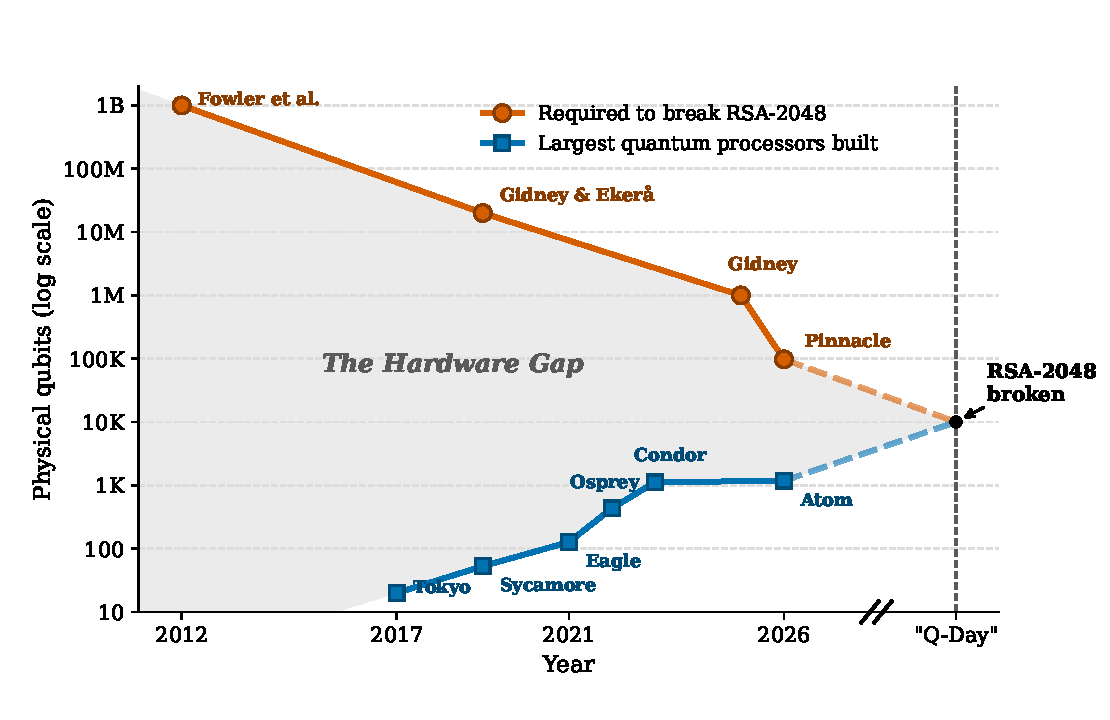
\includegraphics[width=0.85\textwidth]{figures/chapter1/hardware_gap.pdf}
    \caption{The hardware gap for factoring RSA-2048. The descending trend shows
    successive estimates of the physical qubits \emph{required} to factor a
    2048-bit RSA integer~\cite{fowler2012surface,gidney2021factoring,gidney2025how,webster2026pinnacle},
    while the ascending trend shows the largest gate-model quantum processors
    actually \emph{built}~\cite{arute2019quantum}. The two are not a like-for-like
    comparison: achieved counts are noisy physical qubits, whereas the required
    counts assume fault-tolerant physical qubits with error correction (physical
    error rate $\approx 10^{-3}$). The shaded region is the hardware gap, which has
    narrowed over time. To illustrate when this gap might close, the dashed lines show
    a stylized extrapolation towards a hypothetical ``Q-Day''.}
    \label{fig:hardware_gap}
\end{figure}

\subsection{The Dual Path to Quantum Resilience}

If a large-scale CRQC remains years away, why must communication infrastructure change today? The imperative is driven by ``Harvest Now, Decrypt Later'' (HNDL) attacks, where adversaries intercept and store encrypted traffic today, intending to decrypt it once quantum hardware matures~\cite{blanco2026practical}.

The urgency of this threat depends fundamentally on information value decay. Capturing, securely storing, and eventually processing petabytes of traffic on early fault-tolerant quantum computers will be astronomically expensive. Because not all secrets are created equal, this economic reality creates a natural divergence in how data must be protected. High-decay data, such as e-commerce transactions or session tokens, lose their value within minutes. By the time a CRQC is available, their residual value is effectively zero. In contrast, low-decay data, such as state secrets, genomic databases, or critical intellectual property, can retain immense value for decades, making them viable targets for long-term archiving today.

Defending against this threat relies on two fundamentally different paradigms: PQC and QKD.
PQC replaces vulnerable algorithms like RSA and elliptic curve cryptography with new computational problems, such as lattice- or hash-based cryptography, that are believed to be hard for both classical and quantum computers. Its primary advantage is scalability. PQC operates over existing classical networks. However, its security still rests on unproven mathematical assumptions. The unexpected collapse of candidate algorithms like SIKE highlights this risk~\cite{castryck2023sidh}. Building true confidence in new computational primitives requires years of intense cryptanalytic scrutiny.

In contrast, QKD offers information-theoretic security grounded in the laws of quantum mechanics. Because any attempt to eavesdrop on quantum states inevitably disturbs them, QKD provides a mathematically provable guarantee of secrecy that is immune to algorithmic breakthroughs or infinite computational power. While this theoretical guarantee is absolute, practical implementations remain vulnerable to hardware side-channels. Furthermore, its deployment comes at a steep practical cost. It requires specialized photonic hardware, dedicated optical channels, and complex control systems, making it difficult to scale.

Because data spans a vast spectrum of value and lifespan, a uniform defense is both economically and architecturally impractical. The massive volume of high-decay data requires the scalable deployability of PQC. Unconditionally high-value, low-decay secrets demand the eternal security of QKD. Between these poles, a protracted transition period requires crypto-agility and the flexible combination of multiple cryptographic mechanisms to hedge against potential algorithmic failures. Modern networks must therefore support a heterogeneous cryptographic ecosystem.

\section{Scope and Contributions}

\subsection{The Cross-Layer Imperative}

Recognizing the need for both PQC and QKD is only the first step; deploying them exposes a deeper architectural crisis. Neither solution can simply be dropped into existing systems as a software update.

PQC introduces significantly larger key sizes, heavier signatures, and complex arithmetic. When deployed at the scale of modern datacenters, these algorithms consume excessive CPU cycles and severely degrade network throughput and latency. Restoring performance requires pushing cryptographic operations out of the host processor and into specialized network infrastructure, such as data processing units (DPUs).

Similarly, scaling QKD beyond point-to-point physics experiments into operational infrastructure is an immense engineering challenge. It requires miniaturizing bulk optical components onto integrated photonic chips, designing high-throughput real-time post-processing pipelines to distill secure keys, and interfacing these quantum systems with classical network stacks.

Consequently, mitigating the quantum threat is not merely an algorithm selection problem---it is a fundamental integration challenge. A cryptographic primitive that is secure in theory is useless if it violates the latency, throughput, power, or observability constraints of the network. Scalable quantum-resilient communication therefore demands a \emph{cross-layer} approach, requiring systems to be co-designed across the device layer (integrated photonics and physical channels), the protocol layer (QKD post-processing and post-quantum algorithms), and the infrastructure layer (programmable networks, datacenter transport, and observability).

\subsection{The QUARC Project}

The work in this dissertation was carried out within Quantum Resistant
Communications: Advance Learning in Applied PQC Training (QUARC), a Marie
Sk\l{}odowska-Curie Actions (MSCA) doctoral network funded under Horizon Europe and run
as an industrial doctorate~\cite{QUARC2022,quarcwebsite}. QUARC was established to
train a cohort of doctoral researchers in the practical application of
post-quantum cryptography as the first standardized PQC algorithms moved from
specification toward real-world deployment, with each candidate spending a
substantial share of their time embedded within an industrial partner. For the
research reported here that partner was NVIDIA, and the work was shaped
throughout by close collaboration with its networking organization.

\subsection{Research Questions}

This dissertation is organized around the following research questions.

\begin{tcolorbox}[
    colback=gray!5!white,
    colframe=blue!50!black,
    title=\textbf{Research Questions (RQs)},
    fonttitle=\bfseries,
    sharp corners,
    boxrule=0.8pt]
\begin{enumerate}[label=\textbf{RQ\arabic*:}, leftmargin=1.2cm]
    \item How can PQC workloads be accelerated and
deployed efficiently on programmable network infrastructure?
    \item What architectural choices make QKD systems more scalable and
practical in high-performance datacenter networks?
    \item How can integrated photonic entanglement sources be designed and
characterized for deployable, wavelength-division multiplexed QKD systems?
    \item How do device-level, protocol-level, and infrastructure-level design
choices interact when building scalable quantum-resilient communication
systems?
\end{enumerate}
\label{en:researchquestions}
\end{tcolorbox}

RQ1--RQ3 address three complementary engineering problems: deploying PQC
efficiently, scaling QKD systems, and designing deployable integrated quantum
sources. RQ4 provides the cross-layer synthesis by examining how decisions in
one area constrain or enable the others.

\subsection{Publications and Intellectual Property}

The main body of this dissertation is organized around published manuscripts,
as well as manuscripts currently under review, produced during this PhD.
In addition to these peer-reviewed publications and submissions, the industrial
research undertaken within the QUARC project yielded several patent applications.
While the full technical details of these patents are omitted due to intellectual
property restrictions, their scope maps directly to the focus of this thesis,
and their conceptual role in the overarching architecture is mapped in
Figure~\ref{fig:field-venn}. A complete list of the publications (P1--P9) and
inventions (I1--I4) can be found in the List of Publications.

\section{Structure}

The structure of the dissertation is as follows:

\medskip
\textbf{Chapter~\ref{ch:background}} establishes the cross-layer framework used throughout the dissertation and introduces the DPU as a recurring infrastructure substrate for the offload and observability contributions. Topic-specific background is developed in each paper-centric chapter where it is needed.

\medskip
The core contributions are then divided into three parts:

\medskip
\textbf{Part~I --- Quantum Key Distribution} treats quantum key distribution as a deployable network capability rather than only a point-to-point protocol.
\begin{itemize}
\item \textbf{Chapter~\ref{ch:quantum-sources}} discusses the integrated photonic foundations of practical quantum-secure networking, addresses RQ3, and presents P1 and P2.
\item \textbf{Chapter~\ref{ch:qkd-dpu}} discusses scalable QKD post-processing offload on programmable network hardware, addresses RQ2, and presents P3.
\end{itemize}

\medskip
\textbf{Part~II --- Post-Quantum Cryptography} investigates how post-quantum cryptographic algorithms can be executed efficiently on heterogeneous platforms, collectively addressing RQ1.
\begin{itemize}
\item \textbf{Chapter~\ref{ch:dpu-pqc}} discusses CPU-GPU-DPU workload partitioning and latency tradeoffs for datacenter-scale PQC deployment, addresses RQ1, and presents P4 and P5.
\item \textbf{Chapter~\ref{ch:ai-pipelines}} discusses the application of post-quantum mechanisms to secure end-to-end artificial intelligence (AI) pipelines, addresses RQ1, and presents P6.
\end{itemize}

\medskip
\textbf{Part~III --- Datacenter-Scale Security} widens the lens from individual devices and nodes to the datacenter operating as a whole, and stops treating the shared substrate beneath it as a trustworthy given. It examines that substrate first as an attack surface and then as a defensive vantage point, exposing the cross-layer interactions at the heart of RQ4.
\begin{itemize}
\item \textbf{Chapter~\ref{ch:rdma}} treats the infrastructure as an attack surface, spanning device-level side channels through to the ordering- and timing-related risks of remote direct memory access (RDMA) over high-throughput optical fabrics, addresses RQ4, and presents P7.
\item \textbf{Chapter~\ref{ch:confidential-ai}} inverts that argument into a defence, using cross-layer observability and intrusion detection to protect confidential AI training clusters, addresses RQ4, and presents P8 and P9.
\end{itemize}

\medskip
Finally, \textbf{Chapter~\ref{ch:cross-layer}} synthesizes the cross-layer lessons from the preceding parts to fully resolve RQ4, discussing limitations and the future outlook.

\medskip
While this structure divides the thesis sequentially by technological domain, scalable quantum-resilient communication is an inherently cross-layer challenge. As illustrated in Figure~\ref{fig:field-venn}, these domains are highly entangled in practice. The pairwise overlaps mark where QKD and PQC integrate directly with programmable network hardware, while a multi-hybrid key-exchange architecture draws on all three parts simultaneously.

\begin{figure}[htbp]
    \centering
    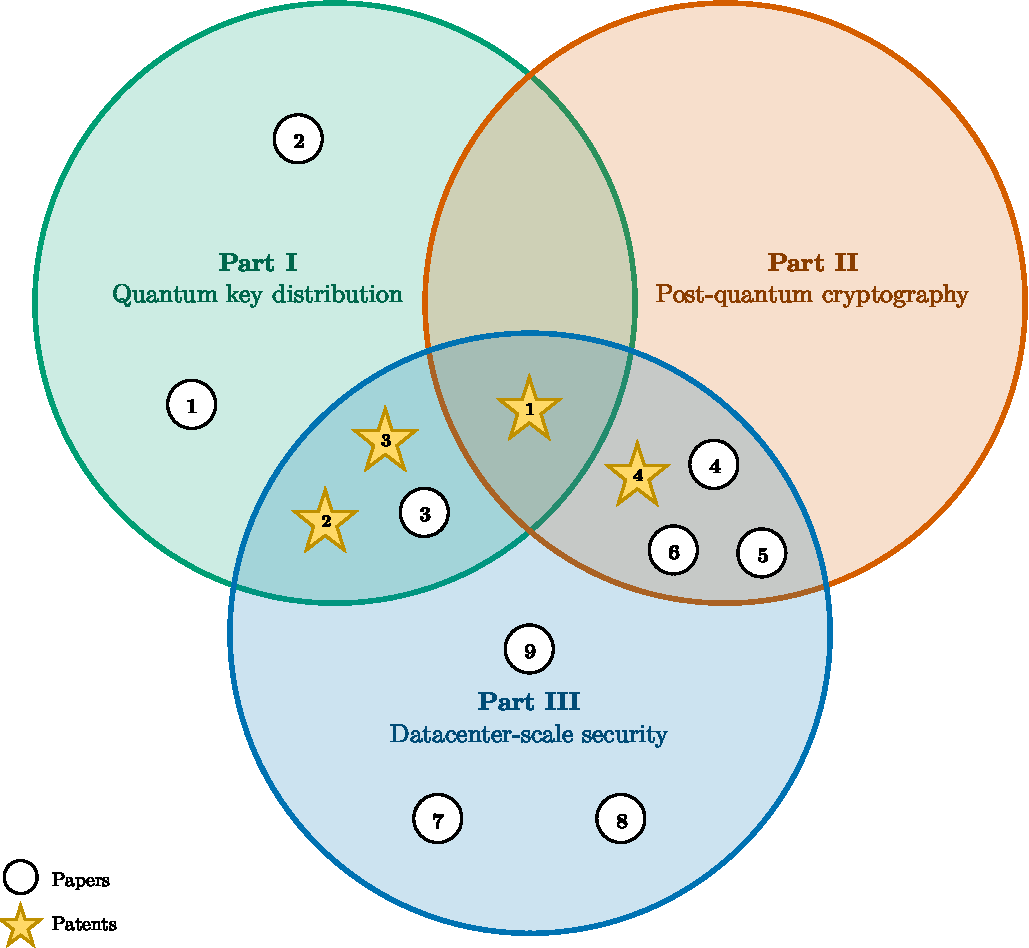
\includegraphics[width=0.7\textwidth]{figures/chapter1/field_venn.pdf}

    \caption{Mapping of the dissertation's contributions onto its three core
    parts. Circular markers denote peer-reviewed papers and star markers denote
    patents.}
    \label{fig:field-venn}
\end{figure}
